\documentclass[10p]{article}
\usepackage[a4paper, total={5.5in, 9in}]{geometry}
\usepackage[leqno]{amsmath}
\usepackage{tikz}
\makeatletter
\newcommand{\leqnomode}{\tagsleft@true\let\veqno\@@leqno}
\newcommand{\reqnomode}{\tagsleft@false\let\veqno\@@eqno}
\makeatother
\usepackage{amssymb}
\usepackage{amsthm}
\usepackage{float}
\usepackage{bbm}
\usepackage{color}
\usepackage{multirow}
\usepackage{booktabs}
\usepackage{algpseudocode}
\usepackage{rotating}
\usepackage{wrapfig}
\usepackage{titling}
\usepackage{authblk} %new
\usepackage{blindtext} %new
\usepackage{breakcites} %break logn citationa
\providecommand{\keywords}[1]{\textbf{\textit{Keywords---}} #1} %keywords
\usepackage[toc,page]{appendix} %appendix package
\usepackage{algorithm}
%\usepackage{hyperref}

\usepackage{hyperref}

\newtheorem{theorem}{Theorem}
\newtheorem{proposition}{Proposition}
\theoremstyle{definition}
\theoremstyle{definition}
\newtheorem{remark}{Remark}
%\theoremstyle{theorem}
\newtheorem{lemma}{Lemma}
\newtheorem{corollary}{Corollary}

\newtheorem{definition}{Definition}
\allowdisplaybreaks

\begin{document}

\setlength{\droptitle}{-4em}   % This is your set screw

\title{Identifying responsibility in a Nigerian sex trafficking network: a game theoretic approach}
%\author{Frank de Meijer \qquad Aras Selvi }
%\author{Aras Selvi}
%\affil{CentER, Department of Econometrics and OR, Tilburg University, The Netherlands }
\author[1]{Frank de Meijer}
\author[2]{Aras Selvi}
\affil[ ]{ CentER, Department of Econometrics and OR, Tilburg University, The Netherlands}
\affil[1]{\textit {\href{mailto:f.j.j.demeijer@tilburguniversity.edu}{f.j.j.demeijer@tilburguniversity.edu}}}
\affil[2]{\textit {\href{mailto:a.selvi@tilburguniversity.edu}{a.selvi@tilburguniversity.edu}}}

%\date{\today}
\date{}

\maketitle

\begin{abstract} \noindent
In this work, we investigate a popular network problem arising in the criminal sciences as well as psychological studies. We consider a Nigerian-Italian sex trafficking network and we are interested in finding the most effective members in this network. Instead of applying classical social network analysis, we introduce a game theoretic setting to this problem. In order to model the effectiveness of a subset of the players, we propose two types of cooperative games. By using Operations Research techniques we approximate the Shapley value: a measure of importance of a `player' in a cooperative game based on marginal contributions. 
\end{abstract}
\keywords{Human trafficking networks, Shapley value, weighted connectivity game, weighted local game}

\reqnomode

\section{Introduction}
Thousands of West-African sex-trafficking victims are arriving to Europe every year \cite{morselli2009inside}. These victims, exclusively women, are forced to prostitution and other forms of sexual exploitation. The authors of \cite{olagbegi2006human} show that most of these victims are from Nigeria, since the majority of crime networks in Nigeria are based on sex-trafficking for various reasons (unemployment, persuasion via rituals, threatening, etc.). The paper \cite{mancuso2014not} studies a police investigation named `Foglie nere' which had issued arrest warrants of Nigerian sex trafficking networks in 2009. This case is significantly important, because it focuses on Nigeria based victims of sex trafficking in Italy. 72\% of the West-African sex network victims are detected in Italy from 2003 to 2007, and the Nigerian victims were by far the majority \cite{morselli2009inside}. Therefore, the `Foglie nere' case is a very reliable example of such sex trafficking networks. \\  \\
Details about the organization of the network can be found in the work \cite{mancuso2014not}. These include the way victims are dragged into the network, the way they are placed in European countries, transportation modes, destination countries, visa processes, etc. We focus on the network of `Foglie nere', where nodes belong to one of different types. The node types are: \textit{Responsible for control, Victims-madams, Madams, Traffickers, Victims, Other roles}. The first type, \textit{Responsible for control} are involved in the direct exploitation of the victims, and they are responsible for the connection between the victims and madams. \textit{Madams} are the ones (usually in Nigeria), who `own' victims. Similarly, \textit{Victims-madams} are the persons who are active victims and madams at the same time. The \textit{Traffickers} are responsible for the logistics and documentation work. Finally, the \textit{Other roles} are persons who are in close touch with the network but have different duties. The full sex trafficking network that we study can be found in \cite{mancuso2014not}. In this network all actors are included as nodes and an edge between them is included whenever the two actors communicate.

The goal of this work is to identify which of the actors are most responsible for the harm caused by the network. In \cite{mancuso2014not} standard social network analysis is applied to complete this task, e.g., by calculating centrality measures such as the betweenness and the intra-group density, see \cite{wasserman1994social}. A drawback of these classical centrality measures is that they only take into account the network structure. In this work we introduce two new centrality measures based on a game theoretic approach. A similar approach is used to rank the players in a terrorist network, see \cite{lindelauf2011game, husslage2015ranking, campen2018new}. This method outperforms classical centrality measures, since it enables the incorporation of additional information on the players and their connections in the analysis.

This paper is organized as follows: In section 2 we provide additional information on the data that we use for our analysis. In Section 3 we define two types of cooperative games that represent the effectiveness of each subset of the players and we describe how to approximate the Shapley value for these games. After this, in Section 4 we present and discuss the rankings based on the new centrality measures. Finally, in Section 5 we conclude the work and add some future research ideas.

\section{Data}
Before we are able to put the sex trafficking network in a game theoretic setting, we look closer to the original data. The original network constructed in \cite{mancuso2014not} consists of 86 actors, among which 8 madams, 2 victim-madams, 31 responsible for control (from now on called controllers), 18 traffickers, 8 other roles and 19 victims. Each victim is only connected to a single other node in the network, either a madam, victim-madam or a controller. The actor corresponding to this node can be seen as the `owner' of the victim, i.e., the person directly responsible for this victim. Since the victims are not held responsible for the committed crimes, these are not considered players in the cooperative games. Instead, we introduce a weight function on the remaining nodes that represents the number of victims that it is connected to. This weight function is formally introduced in Section \ref{GameTheoreticalSetting}. Moreover, we do not take traffickers and other roles into account, since preliminary studies (see e.g., \cite{mancuso2014not}) show that these roles have a small impact on the effectiveness of the network. Finally, for simplicity, the victims-madams are treated as madams that are responsible for one additional victim, namely herself. These adaptations result in a network of 41 actors, among which 31 controllers and 10 madams. The updated network can be found in Appendix \ref{AppendixNetwork}. This network is used to define the game theoretic centrality measures introduced in the next section.

\section{Game Theoretic Setting} \label{GameTheoreticalSetting}
In this section we put the sex trafficking network in a game theoretic setting by defining two types of games that represent the effectiveness of the various coalitions in the network. Moreover, we describe how the Shapley value \cite{shapley1953value} can be approximated and used to identify the responsibility of each player in the network. \\ \\
Let $M$ denote the set of madams and let $C$ denote the set of controllers ($M \cap C =\emptyset$). Together, these sets form the set of players (i.e., actors in the network), which we denote by $N$. For each $i \in N$, we let $d_i$ denote the number of victims for which player $i$ is directly responsible. 

A network can be interpreted as an undirected graph $G = (N,E)$ with vertex set $N$ and edge set $E$. Note that each vertex in $G$ represents a madam or a controller. If two players communicate, we connect their corresponding vertices by an edge. For each subset $S \subseteq N$, let $G[S] = (N[S], E[S])$ denote the subgraph of $G$ induced by the players in $S$. Moreover, for all $i \in N$ let $\delta(i)$ denote the set of neighbours of player $i$, i.e., $\delta(i) = \{ j \in N \, : \, \, (i,j) \in E\}$.

Before we construct a game, we define a weight function $w : N \rightarrow \mathbb{R}$ that represents the individual responsibility or effectiveness of a player. An obvious choice would be $w_i = d_i$ for all $i \in N$. Since most of the controllers work as intermediates, it follows that $d_i = 0$ for most of these players. This might underestimate the direct responsibility of the controllers, since in many cases the controllers are indispensable for the effectiveness of a network (see e.g., \cite{mancuso2014not}). For that reason, we define a control parameter $\alpha \in [0,1]$ and define a weight function $w^\alpha$ as follows:
\begin{align*}
    w^\alpha_i = \begin{cases} d_i & \text{if $i \in M$,} \\d_i + 
    \alpha \sum_{j \in \delta(i)}d_j & \text{if $i \in C$.}
    \end{cases}
\end{align*}
The intuition behind this function is that the controllers are held partly responsible for the victims of their neighbours, depending on the control parameter $\alpha$. If $\alpha$ is close to 1, then the controllers are heavily responsible for its neighbours' victims, while $w^\alpha = d$ if $\alpha = 0$.

Note that the weight function $w^\alpha$ only measures direct responsibility of the players and does not take into account the centrality of the network. To measure this latter quantity as well, we construct a game corresponding to the network.\\ \\
A cooperative game is represented by the pair $(N,v)$, where $N$ equals the set of players and $v : 2^N \rightarrow \mathbb{R}$ assigns a value to each coalition $S \subseteq N$. The value $v(S)$ can be seen as a measure for the effectiveness of the sub-network $G[S]$ induced by the players in $S$. The value of the grand coalition, $v(N)$, can be seen as the total effectiveness of the network. A main question in cooperative game theory is how to allocate the total effectiveness $v(N)$ among the players, i.e., which of the players are most important for the success of the network? We use a well-known solution concept known as the Shapley value \cite{shapley1953value}, which is based on the players' marginal contributions to the coalitions.

Before we compute the Shapley value, the main question is how to define $v$ such that it represents the effectiveness of a coalition in the best way. In the next sections, we propose two different settings.

\subsection{Weighted connectivity game}
A reasonable measure for the centrality of a (sub-)network is its connectivity, since a cell in the network has more strength if the players directly communicate with one another. Based on a similar approach of \cite{husslage2015ranking}, we let $v_1^\alpha(S)$ be equal to the largest weighted connected component in $G[S]$. This yields the following weighted connectivity game $v^\alpha_1$:
\begin{align*}
    v_1^\alpha(S) = \max_{\substack{T \subseteq S : \, G[T] \\ \text{connected}}}\quad \sum_{i \in T}w^\alpha_i \qquad \text{for all $S \subseteq N$.} 
\end{align*}
One can easily verify that the corresponding game $(N, v_1^\alpha)$ is monotonic for all $\alpha \in [0,1]$. Namely, if $S_1 \subseteq S_2$ and $T$ is the largest weighted connected component in $S_1$, then also $T \subseteq S_2$. Consequently, we know that $v_1^\alpha(S_2) \geq \sum_{i \in T}w^\alpha_i = v_1^\alpha(S_1)$.

\subsection{Weighted local game}
The assumption behind the weighted connectivity game is that the effectiveness of a sub-network only depends on its largest weighted connected component. This assumption might be too radical. Namely, in the case of sex trafficking networks it is possible for two sub-networks to operate independently from one other provided that each sub-network consists of sufficient members. This leads to a so-called weighted local game, in which a coalition $S$ incurs the weights of its players for which all its neighbours are also in $S$. We define $v_2^\alpha$ as:
\begin{align*}
    v_2^\alpha (S) = \sum_{i \in S : \delta(i) \subseteq S} w_i^
    \alpha \qquad \text{for all $S \subseteq N$.}
\end{align*}
The intuition behind this function is that if a player $i$ and all its neighbours are included in $S$, then the sub-network centered around $i$ can operate and, thus, is effective. One can easily verify that $(N,v_2^\alpha)$ is monotonic. Moreover, we show that this game is convex.

\begin{theorem}
The game $(N,v_2^\alpha)$ is convex for all $\alpha \in [0,1]$.
\end{theorem}
\begin{proof}
Let $S, T \subseteq N$. In order to show that $(N,v_2^\alpha)$ is convex, we need to show that we have $v(S \cup T) + v(S \cap T) \geq v(S) + v(T)$. Since $S \cup T = (S \setminus T) \cup (S \cap T) \cup (T \setminus S)$, we have
\begin{align*}
    v_2^\alpha(S \cup T) + v_2^\alpha(S \cap T) & = \sum_{\substack{i \in S \cup T : \\ \delta(i) \in S \cup T}}w_i^\alpha \,\, + \sum_{\substack{i \in S \cap T : \\ \delta(i) \in S \cap T}}w_i^\alpha \\
    & = \sum_{\substack{i \in S \setminus T : \\ \delta(i) \in S \cup T}}w_i^\alpha \,\,+ \sum_{\substack{i \in S \cap T : \\ \delta(i) \in S \cup T}}w_i^\alpha \,\,  + \sum_{\substack{i \in T \setminus S : \\ \delta(i) \in S \cup T}}w_i^\alpha \, \, + \sum_{\substack{i \in S \cap T : \\ \delta(i) \in S \cap T}}w_i^\alpha.
\end{align*}
We can now establish a lower bound on the second term by observing that for all $i \in S \cap T$ with $\delta(i) \subseteq S$ or $\delta(i) \subseteq T$, we have $\delta(i) \subseteq S \cup T$. Hence,
\begin{align*}
    \sum_{\substack{i \in S \cap T : \\ \delta(i) \in S \cup T}}w_i^\alpha & \geq \sum_{\substack{i \in S \cap T : \\ \delta(i) \in S}}w_i^\alpha + \sum_{\substack{i \in S \cap T : \\ \delta(i) \in T}}w_i^\alpha \,\, - \sum_{\substack{i \in S \cap T : \\ \delta(i) \in S \cap T}}w_i^\alpha.
\end{align*}
Combining the results above, we obtain
\begin{align*}
    v_2^\alpha(S \cup T) + v_2^\alpha(S \cap T) & \geq \sum_{\substack{i \in S \setminus T : \\ \delta(i) \in S \cup T}}w_i^\alpha + \sum_{\substack{i \in S \cap T : \\ \delta(i) \in S}}w_i^\alpha  + \sum_{\substack{i \in S \cap T : \\ \delta(i) \in T}}w_i^\alpha + \sum_{\substack{i \in T \setminus S : \\ \delta(i) \in S \cup T}}w_i^\alpha \\
    & \geq \sum_{\substack{i \in S : \\ \delta(i) \in S}}w_i^\alpha + \sum_{\substack{i \in T : \\ \delta(i) \in T}}w_i^\alpha = v_2^\alpha(S) + v_2^\alpha(T).
\end{align*}
We conclude that $(N,v_2^\alpha)$ is convex. 
\end{proof}
Since each convex game is totally balanced, it follows that $(N,v_2^\alpha)$ is totally balanced and that the Shapley value of this game belongs to the core of the game. For details and properties of the core see e.g., \cite{borm2001operations}.

\subsection{Approximation of the Shapley value}
The Shapley value is a solution concept for a game $(N,v)$ that is based on marginal vectors. Let $\Pi$ denote the set of all permutations of the set of players. For a given ordering $\sigma \in \Pi$, if player $i$ is on position $k$, then the marginal contribution of player $i$ in $\sigma$ equals $m_v^\sigma(i) = v(\{\sigma_1, ..., \sigma_k\}) - v(\{\sigma_1, ..., \sigma_{k-1}\})$. The Shapley value $\Phi_i(v)$ for player $i$ is the average marginal contribution of player $i$ over all orderings in $\Pi$, i.e., $\Phi_i(v) = \frac{1}{|N|!}\sum_{\sigma \in \Pi}m_v^\sigma (i)$. 

In our case, $|N| = 41$, which implies that we need to consider $41! \approx 3.35 \cdot 10^{49}$ orderings. Because of this, it is not possible to compute $\Phi(v)$ exactly. Instead, we make use of an approximation method proposed by \cite{campen2018new} which is called structured random sampling. Let $t$ be some positive integer, then the procedure works as follows:
\begin{itemize} \itemsep0em 
    \item Select a subset $\Pi_r$ of $\Pi$ with $r = t \cdot |N|$;
    \item Divide the subset $\Pi_r$ in $|N|$ groups of size $t$;
    \item For all players $i \in N$, do:
    \begin{enumerate} \itemsep0em 
        \item Swap player $i$ with the player at position $j$ for each of the $t$ orderings in group $j$, where $j \in \{1, ..., |N|\}$, resulting in a set $\Pi_r'$ of $r$ new orderings;
        \item Compute the marginal contributions $m_v^\sigma(i)$ of player $i$ for all $\sigma \in \Pi_r'$;
        \item Calculate $\hat{\Phi}_i(v) = \frac{1}{r !}\sum_{\sigma \in \Pi_r'}m_v^\sigma(i)$.
    \end{enumerate}
\end{itemize}


\section{Computation and Results}
In this section, we apply our game theoretic centrality measures to the network at hand and discuss the main findings. \\ \\
In the previous section we introduced two types of game theoretic centrality measures, namely $\hat{\Phi}(v_1^\alpha)$ and $\hat{\Phi}(v_2^\alpha)$. The first is mainly based on connectivity (i.e., the effectiveness of a coalition is represented by the largest connected sub-network), while the second is based on the number of local networks (i.e., an actor in the network can operate if all its neighbours are also in the coalition). Both measures still depend on the control parameter $\alpha$, which counts for the direct responsibility of the controllers. Since there is no data on the value of $\alpha$, we calculate $\hat{\Phi}(v_1^\alpha)$ and $\hat{\Phi}(v_2^\alpha)$ for various values of $\alpha$ to see how the rankings depend on $\alpha$. In Appendix $\ref{AppendixValues}$ the measures $\hat{\Phi}(v_1^\alpha)$ and $\hat{\Phi}(v_2^\alpha)$ are calculated for $\alpha = 0, 0.4, 0.6$ and $1$. We also report the betweenness centrality measure of \cite{mancuso2014not}. In Appendix $\ref{AppendixRankings}$ we compare the rankings we obtain from our centrality measures with the ranking of \cite{mancuso2014not}, again for multiple values of $\alpha$. We used $t = 250$ in the approximation of the Shapley values. Preliminary experiments have shown that for $t \geq 100$ only minor changes occur in the rankings. Using $t = 250$, the calculation of a single centrality measure can be done within 100 seconds at a standard PC.\footnote{The PC has an 8-th Generation Intel(R) Core(TM) i7-8750H processor}  We use Python 3.7 \cite{Rossum:1995:PRM:869369} as the main programming language, and develop in the Jupyter Notebook platform \cite{Kluyver:2016aa}. Array operations are done with the package NumPy \cite{numpy}, graph operations are done with the package NetworkX \cite{team2014networkx}, and for the visual plotting we use Matplotlib \cite{Hunter:2007}. The project repository is publicly available on \textit{GitHub}\footnote{\url{https://github.com/arasselvi/Nigerian-Sex-Trafficking-O.R.}}. \\ \\
If we look at the measure $\hat{\Phi}(v_1^\alpha)$, we see that the rankings are quite robust with respect to the value of $\alpha$. The rankings for $\alpha = 0.6$ and $\alpha = 1$ are completely identical and for lower values there are only some minor differences. In general, we see that if the value of $\alpha$ increases, the vertices that fulfill a brokerage position (e.g., player 14 and 18) become more important. Indeed, an increase of $\alpha$ results in a larger total weight of a connected component and thus in a relative increase of the marginal contributions of the players that fulfill a brokerage position. In general, the players 10, 26, 14, 21 and 23 can be seen as most dangerous in the network. These are exactly the five players in the top 5 ranking of \cite{mancuso2014not}. 

Next, we look at the measure $\hat{\Phi}(v_2^\alpha)$. The rankings resulting from this measure are less robust against the value of $\alpha$. If $\alpha$ increases, then the players with a large number of high-weighted neighbours become more important. Although the rankings are less robust than those of $\hat{\Phi}(v_1^\alpha)$, there are several players that appear in the top-5 for all considered values of $\alpha$, namely player 26, 10, 3, 8 and 2. If we look at the graph, these are indeed the players that have a large and/or high-weighted local network centred around them. It has to be noted that players that have a low weight, but are at a brokerage position (e.g., player 18, 21 and 23) appear in a very low position in the ranking. This is due to the underlying assumption of this centrality measure, which values the effectiveness of sub-networks instead of taking into account the connectivity. 

In Table \ref{TableAverageRankings} the top-5 ranking based on our game theoretic centrality measure averaged over $\alpha$ is presented. Moreover, we include the ranking based on the betweenness centrality measure of \cite{mancuso2014not}.
\begin{table}[H]\centering
\begin{tabular}{*{3}{c}}
\toprule
\cite{mancuso2014not}
 & $\hat{\Phi}(v_1^\alpha)$ & $\hat{\Phi}(v_2^\alpha)$ \\
\midrule
10 & 10 & 26 \\ 
26 & 26 & 10\\ 
23 &14 & 8 \\ 
21 & 21& 3 \\ 
14 & 23& 2 \\ 
\bottomrule
\end{tabular}
\caption{Average rankings of $\hat{\Phi}(v_1^\alpha)$ and $\hat{\Phi}(v_2^\alpha)$ over $\alpha$ and the ranking from \cite{mancuso2014not}. \label{TableAverageRankings}}
\end{table}

\noindent Considering both measures, we conclude that player 10 and 26 can be seen as most responsible for the effectiveness of the network. These players are both madams. The fact that these players have high Shapley values for both introduced centrality measures, shows that these have high-weighted local sub-networks and fulfill a brokerage position in the network. Surprisingly, they are exactly the madams being most active at the overseas operations, i.e., the ones having the most contact with people outside Italian borders (see \cite{mancuso2014not}). 

Moreover, we can conclude that the ranking resulting from the connectivity game are quite similar to the standard centrality measures of \cite{mancuso2014not}. These rankings mainly identify players with a brokerage position in the network. However, the ranking based on the weighted local game gives more insight in the effective sub-networks that can operate independently from the other coalitions. Under the assumption that sub-networks can still operative locally, this method identifies effective players that could not be recognized by the standard centrality measures. 

\section{Conclusion and Future Research}
In this work, we introduced two new game theoretic centrality measures to identify the effectiveness of players in a Nigerian sex trafficking network. In the first game, the effectiveness of a coalition is measured by considering the largest weighted connected component in the sub-network spanned by the coalition. The second game is a so-called weighted local game, where the effectiveness of a coalition is proportional to the total number of local sub-networks that are induced by the players in the coalition. We proved that this latter type of game is convex. By approximating the Shapley value of these games, we can identify the individual responsibility of each player in the network. These methods can be applied successfully to obtain a ranking of the madams and controllers in the sex trafficking network. However, the focus of these rankings is different. It turns out that the first game could be used to identify the players having a brokerage position in the network, while the second game finds the players that fulfill a powerful local position. This latter type of effectiveness could not be measured by the standard centrality measures provided in \cite{mancuso2014not}.\\ \\
The introduced game theoretic centrality measures can be applied to other sex trafficking networks (or similar social networks) as well. For example, \textit{child sex trafficking} would be a candidate area having many network data available \cite{cockbain2018offender}. Recall that our analysis is based on a control parameter $\alpha$ which represents the direct responsibility of the controllers. It would be interesting to have more information about a structured tuning of this parameter. This can be a topic for future research. Moreover, although the weighted connectivity game and the weighted local game have different focuses, both provide useful information about the players in the network. Therefore, it is interesting to also look at other types of value functions that model the effectiveness of a coalition.


\bibliographystyle{apalike}
\bibliography{sample}
\newpage

\begin{appendices}\pagenumbering{Roman} 
\section{Network Figure}  \label{AppendixNetwork}
\begin{figure}[ht]
\centering
    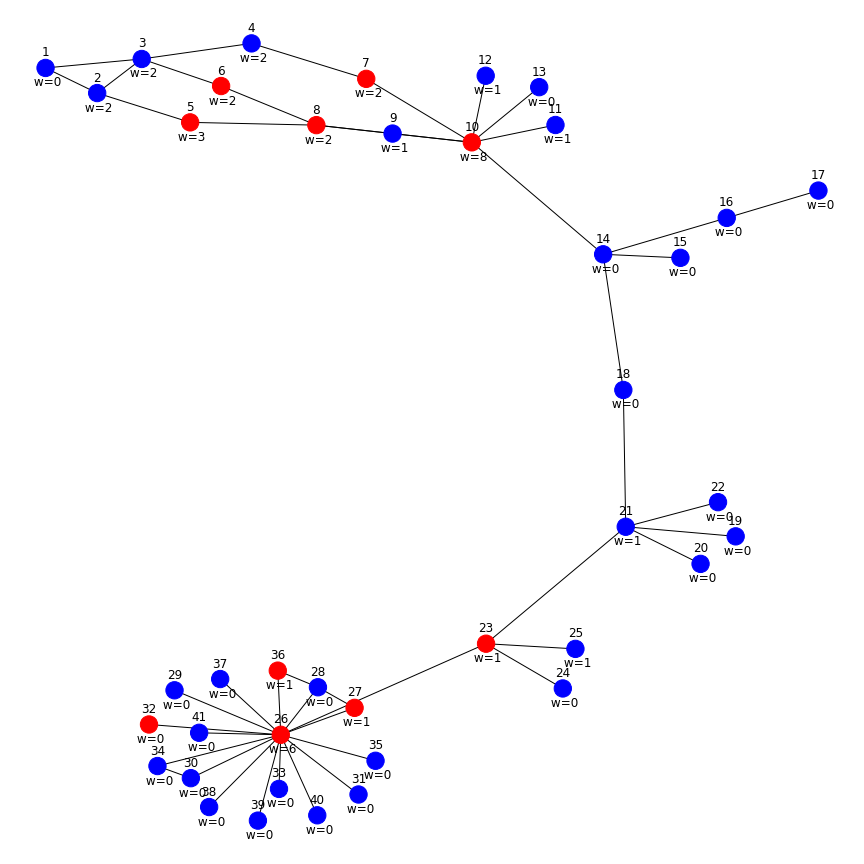
\includegraphics[angle=0,scale=0.5]{network.png}%<---angle here
    \caption{Sex trafficking network. Blue nodes are `responsible for control', red nodes are `madams'. Node indexes are written above a node, while the weight is written just below the node in form, e.g., $w=3$.}
    \label{fig:PropProf}
\end{figure}
\newpage 
\section{Full results} \label{AppendixValues}
The node indexing we used is slightly different than in the paper \cite{mancuso2014not}. Therefore, we share the results with the node indexes in the original paper. Moreover, the indexes with a (*) sign correspond to madams, the others correspond to controllers.
\begin{table}[!ht]\centering
\begin{tabular}{lcccccc}
\toprule
\multirow{2}[3]{*}{Index} & \multirow{2}[3]{*}{\cite{mancuso2014not} Index} &  \multirow{2}[3]{*}{Betweenness Cent.} &\multicolumn{2}{c}{Shapley $\alpha = 0$} & \multicolumn{2}{c}{Shapley $\alpha = 0.4$} \\
\cmidrule(lr){4-5} \cmidrule(lr){6-7}
 & & & $\hat{\Phi}(v_1^\alpha)$ & $\hat{\Phi}(v_2^\alpha)$ & $\hat{\Phi}(v_1^\alpha)$ & $\hat{\Phi}(v_2^\alpha)$ \\
\midrule
1 & N03 & 0.000 & 0.000  &0.901 & 0.442 & 2.282 \\ 
 \hline
 2 & N02 & 11.527 & 1.401 &1.895 & 2.231 & 3.271\\
 \hline
 3 & N01 & 13.999 & 1.936 &2.223 & 3.170 & 4.003\\
 \hline
 4 & N04 & 0.889 & 1.694& 1.713& 2.140 & 2.605\\
 \hline
 5* & N44 & 9.946 & 2.163& 1.894 & 1.842 & 2.359\\
 \hline
 6* & N06 & 2.353 & 1.498&1.464 & 1.364 &1.847\\ 
 \hline
 7* & N18 & 0.000 & 1.993& 2.307& 1.979 & 2.653 \\
 \hline
 8* & N05 & 31.064 & 3.089 &3.358 & 3.140 & 4.613\\
 \hline
 9 & N07 & 0.000 & 0.669& 1.700& 2.807 & 3.006 \\
 \hline
 10* & N16 & 61.755 & 9.661& 3.357&14.800 &  9.821\\
 \hline
 11 & N45 & 0.000 & 0.561& 1.480& 1.982 & 3.002 \\ 
 \hline
 12 & N19 & 2.353 & 0.561&1.480 & 1.982 & 3.002 \\
 \hline
 13 & N46 & 0.000 & 0.000 &0.982& 1.439 &2.498 \\
 \hline
 14 & N20 & 53.782 & 1.933& 0.982& 9.559 & 2.905 \\
 \hline
 15 & N54 & 0.000 & 0.000&  0.000 & 0.000 & 0.600 \\
 \hline
 16 & N52 & 2.353 & 0.000&  0.000& 1.651 &  1.913 \\ 
 \hline
 17 & N53 & 0.000 & 0.000&  0.000& 0.000 & 1.287 \\
 \hline
 18 &  N10 & 50.588 & 1.956 &0.170 & 6.812 & 0.860\\
 \hline
 19 & N85 & 0.000 & 0.000 & 0.170 & 0.000 & 0.165\\
 \hline
 20 & N11 & 0.000 & 0.000 & 0.170 &0.000 & 0.165 \\
 \hline
 21 & N08 & 55.014 & 2.080 & 0.365 & 6.853 & 0.820 \\
 \hline
 22 & N86 & 0.000 & 0.000 & 0.170 &0.000 &0.165 \\
 \hline
 23* & N12 & 55.168 & 1.964 &1.222 & 6.718 &1.355 \\
 \hline
 24 & N15 & 0.000 & 0.000&0.196& 0.000 &0.205 \\
 \hline
 25 & N84 & 0.000 & 0.298 & 0.688 & 0.311 &  0.707\\
 \hline
 26* & N24 & 58.025 & 3.080& 1.210& 10.929 & 14.016 \\
 \hline
 27* & N34 & 0.000 & 0.323& 0.683 & 0.381 & 1.438\\
 \hline
 28 & N28 & 0.014 & 0.001& 1.011 & 1.170 & 1.765\\
 \hline
 29 & N25 & 0.000 & 0.000&0.355 & 0.766 & 1.355 \\
 \hline
 30 & N26 & 0.000 & 0.000&0.355 & 0.776 & 1.673 \\
 \hline
 31 & N39 & 0.000 & 0.000&0.355 & 0.766 & 1.355 \\
 \hline
 32* & N36 & 0.000 & 0.000& 0.355& 0.000 &0.355 \\
 \hline
 33 & N31 & 0.000 & 0.000& 0.355& 0.767 & 1.355 \\
 \hline
 34 & N30 & 0.042 & 0.000 &0.355 & 0.780 &1.684 \\
 \hline
 35 & N38 & 0.000  & 0.000&0.355 &0.767 & 1.355\\
 \hline
 36* & N35 &0.014 & 0.324&0.689 & 0.377 & 1.446 \\
 \hline
 37 & N74 & 0.000 & 0.000 &0.355 & 0.768 &1.355 \\
 \hline
 38 & N77 & 0.000  & 0.000& 0.355& 0.768 &1.355 \\
 \hline
 39 & N80 & 0.000 & 0.000 & 0.355&0.768 &1.355 \\
 \hline
 40 & N79 & 0.000 & 0.000& 0.355&0.768  &1.355 \\
 \hline
  41 & N78 & 0.000 & 0.000 & 0.355&0.768 &1.355 \\
 \hline
\bottomrule
\end{tabular}
\end{table}
\begin{table}[!ht]\centering
\begin{tabular}{lcccccc}
\toprule
\multirow{2}[3]{*}{Index} & \multirow{2}[3]{*}{\cite{mancuso2014not} Index} &  \multirow{2}[3]{*}{Betweenness Cent.} &\multicolumn{2}{c}{Shapley $\alpha = 0.6$} & \multicolumn{2}{c}{Shapley $\alpha = 1$} \\
\cmidrule(lr){4-5} \cmidrule(lr){6-7}
 & & & $\hat{\Phi}(v_1^\alpha)$ & $\hat{\Phi}(v_2^\alpha)$ & $\hat{\Phi}(v_1^\alpha)$ & $\hat{\Phi}(v_2^\alpha)$ \\
\midrule
1 & N03 & 0.000 &  0.819 &3.033 &  1.588 & 4.681\\ 
 \hline
 2 & N02 & 11.527 & 2.431 &3.986 & 3.373 &5.702 \\
 \hline
 3 & N01 & 13.999 & 3.533 &5.077 & 5.065 &7.353 \\
 \hline
 4 & N04 & 0.889 & 2.464&3.133 & 3.372& 4.251\\
 \hline
 5* & N44 & 9.946 & 1.740&2.577 &1.902 & 3.113\\
 \hline
 6* & N06 & 2.353 &1.309 & 2.030&1.429 & 2.676\\ 
 \hline
 7* & N18 & 0.000 & 1.997&2.972 & 2.320 &3.688 \\
 \hline
 8* & N05 & 31.064 & 3.106  &5.280 &3.718 & 6.647\\
 \hline
 9 & N07 & 0.000 & 3.616 & 3.695& 5.684 & 4.996\\
 \hline
 10* & N16 & 61.755 & 16.706 &13.157 & 22.093&20.337 \\
 \hline
 11 & N45 & 0.000 & 2.358 & 3.496& 4.155 & 5.539 \\ 
 \hline
 12 & N19 & 2.353 &2.358  & 3.496& 4.155& 5.539\\
 \hline
 13 & N46 & 0.000 & 1.837 &2.999 & 3.623 & 5.035\\
 \hline
 14 & N20 & 53.782 &12.493 & 3.969& 19.225 &6.304\\
 \hline
 15 & N54 & 0.000 & 0.000 &0.796 & 0.000 & 1.581\\
 \hline
 16 & N52 & 2.353 & 2.381&2.846 & 4.436  &4.926 \\ 
 \hline
 17 & N53 & 0.000 & 0.000& 1.983& 0.000& 3.344\\
 \hline
 18 &  N10 & 50.588 & 8.927  &1.226 & 14.297 &2.252 \\
 \hline
 19 & N85 & 0.000 & 0.000  &0.335 & 0.321&0.832  \\
 \hline
 20 & N11 & 0.000 &0.000  & 0.335& 0.321& 0.832\\
 \hline
 21 & N08 & 55.014 & 9.377& 1.184& 14.479& 2.358\\
 \hline
 22 & N86 & 0.000 & 0.000 &0.335 & 0.323& 0.830\\
 \hline
 23* & N12 & 55.168 & 9.229 & 1.597& 14.262& 2.363 \\
 \hline
 24 & N15 & 0.000 & 0.000& 0.205& 0.344 & 0.698\\
 \hline
 25 & N84 & 0.000 & 0.332 & 0.711& 0.693&1.196 \\
 \hline
 26* & N24 & 58.025 &15.251 &20.508 & 24.191 & 34.209\\
 \hline
 27* & N34 & 0.000 & 0.411&1.657 & 0.437&2.691 \\
 \hline
 28 & N28 & 0.014 &1.728 & 1.981& 3.592 & 3.026\\
 \hline
 29 & N25 & 0.000 & 1.242& 1.842& 2.597&  3.395\\
 \hline
 30 & N26 & 0.000 & 1.276 &2.636 &2.714& 4.378 \\
 \hline
 31 & N39 & 0.000 & 1.242&1.842 & 2.597&  3.395\\
 \hline
 32* & N36 & 0.000 &0.000 &0.334 &0.000 & 0.347\\
 \hline
 33 & N31 & 0.000 &1.237 & 1.842& 2.600 &3.395 \\
 \hline
 34 & N30 & 0.042 & 1.278 & 2.667&2.716 & 4.406\\
 \hline
 35 & N38 & 0.000  &1.237 & 1.842&2.600& 3.395 \\
 \hline
 36* & N35 &0.014 &0.411 &1.680 & 0.440 &2.737 \\
 \hline
 37 & N74 & 0.000 &1.236 & 1.842& 2.608 & 3.395\\
 \hline
 38 & N77 & 0.000  &1.236 & 1.842&  2.608&3.395 \\
 \hline
 39 & N80 & 0.000 &1.236  & 1.842& 2.608& 3.395 \\
 \hline
 40 & N79 & 0.000 &1.236 & 1.842&  2.608&3.395 \\
 \hline
  41 & N78 & 0.000 &1.236  & 1.842&  2.608&3.395 \\
 \hline
\bottomrule
\end{tabular}
\end{table}
\clearpage
\section{Full Rankings} \label{AppendixRankings}
Below, we share the player rankings in each of the methods (first element is the most effective player). Bold elements have zero score, meaning in the corresponding measure they are the ones having least effectiveness. The bold elements are equally unimportant. Moreover, if consecutive elements have the superscript *, they have the same score.\\
\begin{table}[!ht]\centering
\begin{tabular}{*{9}{c}}
\toprule
\multirow{2}[3]{*}{\cite{mancuso2014not}} &  \multicolumn{2}{c}{Shapley $\alpha = 0$} & \multicolumn{2}{c}{Shapley $\alpha = 0.4$} & \multicolumn{2}{c}{Shapley $\alpha = 0.6$}& \multicolumn{2}{c}{Shapley $\alpha = 1$}\\
\cmidrule(lr){2-3} \cmidrule(lr){4-5} \cmidrule(lr){6-7} \cmidrule(lr){8-9}
 & $\hat{\Phi}(v_1^\alpha)$ & $\hat{\Phi}(v_2^\alpha)$ & $\hat{\Phi}(v_1^\alpha)$ & $\hat{\Phi}(v_2^\alpha)$  & $\hat{\Phi}(v_1^\alpha)$ & $\hat{\Phi}(v_2^\alpha)$ & $\hat{\Phi}(v_1^\alpha)$ & $\hat{\Phi}(v_2^\alpha)$\\
\midrule
10 & 10 & 8 & 10&26 & 10& 26&10 &  26\\ 
26 & 8 & 10 & 26& 10&26 &10 &26 &10\\ 
23 &26 & 7 &14 &8 &14 &8 &14 &3\\ 
21 & 5& 3 & 21&3 & 21&3 &21 &8\\ 
14 & 21& 2 &18 & 2&23 & 2&23 &14\\ 
18 &7 & 5 & 23& 9 & 18&14 &18 &2\\ 
8 & 23& 4 & 3&12 & 9&9 &9 &11\\ 
3 &3 & 9 & 8& 11&3 &12 &3 &12\\ 
2 &18 & 12 &9 &14 &8 &11 &8 &13\\ 
5 &14 & 11 &2 &7 & 2 &4 &2 &9\\ 
6* &4 &  6&4 & 4& 4&1 & 4&16\\ 
12* &6 & 23 &12 &13 &16 & 13&16 &1\\ 
16* &2 & 26 &11 &5 & 12&7 &12 &34\\ 
4 &9 &  28&7 & 1& 11& 16& 11&30\\ 
34 &12 & 13 &5 &16 & 7&34 &7 &4\\ 
28* &11 & 14 & 16& 6&13 & 30&13 &7\\ 
36* &27 & 1 & 13&28 &5 &5 &5 &40\\ 
\textbf{1} &36 &36  & 6&34 &28 & 6&28 &41\\ 
\textbf{7} &25 & 25 & 28& 30 &6 & 17&6 &29\\ 
\textbf{9} &28 & 27 &34 &36 &34 &28 &34 &33\\ 
\textbf{11} &\textbf{17} & 21 &30 &27 &30 & 41&30 &39\\ 
\textbf{13} & \textbf{13}& 30 & 33& 23&31 &29 &31 &38\\ 
\textbf{15} &\textbf{15} & 31 & 35& 41&29 &33 &29 &37\\ 
\textbf{17} &\textbf{16} & 39 & 41&29 &33 & 40&33 &35\\ 
\textbf{19} & \textbf{41}&  38& 39& 39&35 &39 &35 &31\\ 
\textbf{20} &\textbf{19} & 37 & 38& 38&41 & 38&41 &17\\ 
\textbf{22} &\textbf{20} & 35  & 40&37 &40 &37 &40 &5\\ 
\textbf{24} &\textbf{40} & 34 & 37& 40&37 &35 &37 &28\\
\textbf{25} & \textbf{22}& 33 & 29&35 & 38& 31&38 &36\\ 
\textbf{27} &\textbf{24} & 32 & 31&33 &39 & 36&39 &27\\ 
\textbf{29} &\textbf{29} & 41 & 1& 31& 1& 27&1 &6\\ 
\textbf{30} & \textbf{30}& 29 & 27& 17&27 & 23&27 &23\\ 
\textbf{31} &\textbf{31} & 40 & 36& 18&36 &18 &36 &21\\ 
\textbf{32} &\textbf{32} & 24 & 26&21 &25 & 21&25 &18\\ 
\textbf{33} &\textbf{33} & 19 & \textbf{19}&25 &\textbf{15} & 15&\textbf{15} &15\\ 
\textbf{35} &\textbf{34} & 22 & \textbf{24}& 15& \textbf{17}& 25&\textbf{17} &25\\ 
\textbf{37} &\textbf{35} & 18 & \textbf{32}& 32& \textbf{19}&19 &\textbf{19} &19\\ 
\textbf{38} &\textbf{37} &20  & \textbf{22}& 24& \textbf{20}&22 &\textbf{20} &20\\ 
\textbf{39} &\textbf{38} & \textbf{15} & \textbf{20}&22 & \textbf{22}& 20&\textbf{22} &22\\ 
\textbf{40} &\textbf{39} &  \textbf{16}& \textbf{15}&20 &\textbf{24} & 32&\textbf{24} &24\\ 
\textbf{41} &\textbf{1} & \textbf{17} & \textbf{17}& 19& \textbf{32}& 34&\textbf{32} &32\\ 
 \hline
\bottomrule
\end{tabular}
\end{table}
\end{appendices}

\end{document}